\subsection{LBM}
\begin{frame}{lattice-Boltzmann Introduction}
Discretize the continuous 
\end{frame}

\begin{frame}{Bhatnagar-Gross-Krook lattice-Boltzmann Formulation}
\begin{align}
	\underbrace{f_i(\vec{x}+\vec{c}_i, t + 1)  = f_i(\vec{x},t)}_\text{streaming}  + \underbrace{\Omega_i(\vec{x},t)}_\text{collision}
\end{align}

The collision operator is calculated based only on each nodes local information. Using the single-relaxation time BGK approximation the collision is calculated as
\begin{align}
	\Omega_i = -\frac{1}{\tau}\left[f_i(\vec{x},t) - f_i^\eq(\vec{x},t)\right]
\end{align}
Relaxation towards the equilibrium distribution function
\begin{equation}\label{eq:equilib-dist-function}
	f_i^\eq = \rho(\vec{x},t)w_i\left[1+\frac{\vec{u}\cdot\vec{c}_i}{c_s^2} + \frac{(\vec{u}\cdot\vec{c}_i)^2}{2c_s^4} - \frac{\vec{u}^2}{2c_s^2} \right]
\end{equation}

\end{frame}

\begin{frame}
Bounce-back boundary condition
\begin{figure}[t]
	\centering
	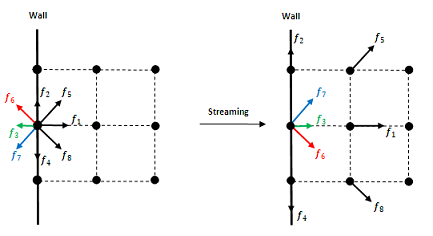
\includegraphics[width=0.5\linewidth]{chapters/figures/lbm/ongrid}\label{fig:wall-lattice-bc}
	\caption{Sketch of the D2Q9 nodes showing at the boundary the distribution functions that would come from neighbors outside the boundary (at the wall) are unknown (drawing from correspondence with Dr. Bao, billbao@cims.nyu.edu).}
\end{figure}
\end{frame}

\begin{frame}
\begin{subequations}\label{eq:lbm2physical}
\begin{align}
	\rho(\vec{x},t) &= \sum_i f_i(\vec{x},t)\\
	\vec{u}(\vec{x},t) &= \frac{1}{\rho(\vec{x},t)}\sum_i \vec{c}_if_i(\vec{x},t)
\end{align}
\end{subequations}

The fluid pressure is related to the density for an ideal gas, so we can find the physical pressure in terms of the lattice density,
\begin{equation}
	p = p_0\frac{\rho(\vec{x},t)}{\rho_0}
\end{equation}
\end{frame}